\chapter{Conclusion}
\label{sec:conclusion}

\dictum{… except in the light of genetics.\par\dictumrule}

\noindent
Evolution by natural selection is the implicit assumption underlying all of
modern biology. \citet{Dobzhansky:1973} famously argues against ill-informed
criticism of evolution, stating

\begin{quote}
    Nothing in biology makes sense except in the light of evolution.
\end{quote}

This statement is as relevant today as it was then --- both as an admonishment
about the still prevalent ignorance of basic biological facts, and serving as a
succinct summary of our understanding of biology. In fact, modern evolutionary
synthesis, which is the prevailing explanatory model employed today, and which
is itself an evolution of the Darwinian theory of descent with modification by
means of natural selection, is unchallenged in this status, and is corroborated
by every new piece of evidence.

In \texttitle{The making of the fittest}, Sean Carroll argues that the best
evidence for evolution we have is the genetic record that we can read in the
\dna of all living species \citep{Carroll:2006}. Carroll was mainly talking
about the similarity between homologous genes in different species. But one of
the most striking examples of strong conservation is the near-universal genetic
code: During billions of years of evolution, the instruction set used to encode
the building blocks of proteins has remained virtually unchanged.

In contrast with the conservation of the genetic code itself, the implementation
of this code shows some degree of variation, most notably in the variation of
the selection of preferential synonymous codons (reviewed in
\citet{Ermolaeva:2001}) on the one hand, and in the divergence of the \trna
genes \citep{Kutter:2011} on the other hand.

In \cref{sec:trna}, I have summarised our research into the variability of the
\trna genes, not across evolution, but across development. Our findings mirror a
common theme: despite pervasive variation of \trna gene expression, the
anticodon isoacceptor \trna abundance remains very stable across different
stages of development, and matches the codon demand of the transcriptome which,
itself, also shows very little variation.

As there is no effect on the abundance of the \trna anticodon isoacceptor pools,
it remains unclear why such variation of the \trna gene expression exists;
however, I have shown that the variation is not stochastic but rather the
product of coordinated regulation, precisely to ensure the stability of the
anticodon pool. As a consequence, this may simply be a stabilising mechanism to
buffer extrinsically caused changes in the expression of individual \trna genes.
The precise mechanism of the \trna gene expression regulation remains unclear
even though I found some evidence of correlation with specific histone marks.

Despite the existence of larger variations in codon usage between subsets of
genes, some of which are cell type specific, I was unable to find evidence for a
regulatory effect of this codon bias on translation rates via higher adaptation
to a cell type specific \trna anticodon isoacceptor pool in mammals. On the
contrary, the variation in the \trna anticodon abundance does not seem to
correlate with cell type specific codon demand. This finding, presented in
\cref{sec:codons} lends support to a view that has recently been challenged
\citep{Gingold:2014,Wilusz:2015}: that translational selection via codon bias,
if present at all, plays a negligible role in mammalian systems. It will be
interesting to see how this controversy will unfold.

I have started exploring other potential sources of the cell type specific codon
bias observed in mammals, which are unrelated to the regulation of translation
rate. My first intuition was that the codon bias might be a stochastic artefact
caused by the small size of the gene sets under consideration. However, while
this does have an effect on codon bias, it is insufficient to explain all the
observed codon bias in most gene sets. I will continue exploring genomic \gc
bias as another potential cause of this effect.

The \pol3 \chipseq data generated for the projects presented in this thesis
provides a wealth of information beyond just \trna gene activity.
\Cref{sec:pol3} takes a brief glimpse at genome-wide \pol3 binding and confirms
previous reports of the association of \pol3 with \transsine loci in vivo.

\section{Future directions}

\subsection{Regulation of \abbr{trna} transcription}

While providing unprecedented insight into the controlled variability of \trna
gene transcription, \cref{sec:trna} has failed to establish a mechanism for the
differential regulation of \trna gene transcription. Known features of \pol3
recruitment, such as transcription factor binding and specific histone marks,
could not conclusively be shown to cause the differences I observed in the \trna
gene transcription between different stages of development. My analysis
deliberately excluded the internal promoters of \trna genes from the search for
specific motifs since it has previously been reported that variation of the
internal promoter of \trna genes is unrelated to variation in gene expression
\citep{Oler:2010,Canella:2012}.

However, results in \citet{Gingold:2014} indicate that this may have been
premature, as they find significant differences in the B box of \trna genes
which they reported as differentially expressed between different conditions.
This suggests that internal promoter variation may contribute to the observed
variability of the \trna transcriptome after all. I intend to run the methods
they used on our data to test this hypothesis.

\subsection{Codon usage adaptation}

The question of what causes codon usage bias variability across functional
subsets of the transcriptome remains wide open. \gc bias, in particular, is
worth exploring further. On the one hand, I observed a robust correlation
between \gc bias and codon usage, and we know that codon usage can sometimes be
predicted from intergenic \gc bias \citep{Chen:2004}. On the other hand,
\citet{Duret:2002} show that, at least in \species{dmel} and \species{cel}, \gc
bias is uncorrelated with codon usage bias.

To explore this further, two avenues present themselves:

\begin{enumerate}
    \item It is known that intergenic isochore \gc content in mammals predicts
        codon usage. Since intergenic regions are non-coding, this suggests that
        differential codon usage between genes has, at best, a minor functional
        relevance. So far, I have only looked at \gc bias in coding sequences.
        To make similar conclusions, I will have to instead compare codon usage
        to the \gc bias in the flanking regions of protein-coding genes.
    \item \gc bias can vary between synonymous and non-synonymous codons. If \gc
        bias is indeed causal for codon usage, we would expect that \gc bias
        correlates highly between the first two nucleotide positions of the
        codon and its wobble position. However, if the wobble position’s \gc
        bias is uncorrelated to the \gc bias of the other codon positions in a
        gene set, this would require a different explanation.
\end{enumerate}

Another feature known to constrain codon deployment is the presence of other
sequence features in the coding region of genes. This includes binding sites for
enhancers and splicing factors \citep{Hyder:1995,Blencowe:2000}. The extent of
this constraint has recently been shown to be much more widespread than
previously assumed \citep{Stergachis:2013}. It is conceivable that condition
specific gene sets carry enhancers for their own transcription in their gene
bodies, which would contribute to a codon usage bias. It would be worthwhile to
investigate the enrichment of such binding sites in gene sets with strong codon
bias, in particular those reported by \citep{Gingold:2014}.

The usage of a simple correlation between matching codons and anticodons,
disregarding wobble base pairing, has proved adequate to demonstrate an overall
high correlation between the codon demand and matching \trna anticodon
isoacceptor pool. However, arguing about the relative adaptiveness of different
gene sets or transcriptomes may make it  necessary to consider wobble base
pairing to model the codon--anticodon interaction more precisely. The \tai
\citep{Dos_Reis:2003} offers a way of quantifying codon--anticodon adaptation by
considering (simplified, see \cref{tab:wobble}) wobble base pairing rules.
However, it is conventionally based on the \trna isoacceptor gene copy number as
a measure of anticodon abundance. I plan to improve this using our \trna gene
expression data, which offer a more accurate anticodon isoacceptor abundance
measure, instead. In addition, it may be possible to extend the \tai metric by
considering extended wobble base pairing rules \citep{Murphy:2004} --- although
it is likely that this will have a very limited effect on the adaptation value.

\subsection{\abbr{Pol3} transcription of \abbr{transsine}s}

The next step in the analysis of \transsine expression requires a framework for
the robust quantification of \pol3 binding signal over background noise. After
this, individual \transsine classes need to be grouped by their \rna gene of
origin. This will allow us to perform a biologically meaningful analysis of
the variation of expression, and will potentially yield insight into the
regulation of related \trna genes.

\clearpage

\begin{center}
    \vspace*{\fill}
    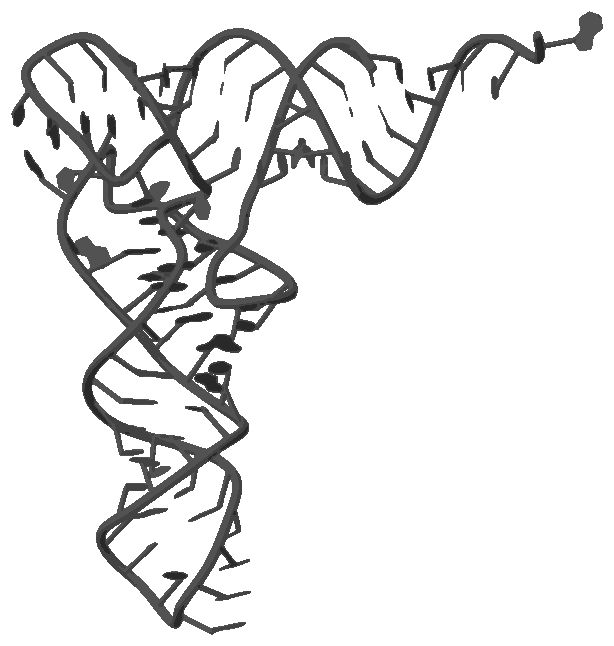
\includegraphics[width=\textwidth]{trna-3d}
    \vspace*{\fill}
\end{center}
